%% For double-blind review submission, w/o CCS and ACM Reference (max submission space)
\documentclass[sigplan,review,anonymous]{acmart}\settopmatter{printfolios=true,printccs=false,printacmref=false}
%% For double-blind review submission, w/ CCS and ACM Reference
%\documentclass[sigplan,review,anonymous]{acmart}\settopmatter{printfolios=true}
%% For single-blind review submission, w/o CCS and ACM Reference (max submission space)
%\documentclass[sigplan,review]{acmart}\settopmatter{printfolios=true,printccs=false,printacmref=false}
%% For single-blind review submission, w/ CCS and ACM Reference
%\documentclass[sigplan,review]{acmart}\settopmatter{printfolios=true}
%% For final camera-ready submission, w/ required CCS and ACM Reference
%\documentclass[sigplan]{acmart}\settopmatter{}


%% Conference information
%% Supplied to authors by publisher for camera-ready submission;
%% use defaults for review submission.
\acmConference[ICFP'19]{ACM SIGPLAN International Conference on Functional Programming}{August 18--23, 2019}{Berlin, Germany}
\acmYear{2019}
\acmISBN{} % \acmISBN{978-x-xxxx-xxxx-x/YY/MM}
\acmDOI{} % \acmDOI{10.1145/nnnnnnn.nnnnnnn}
\startPage{1}

%% Copyright information
%% Supplied to authors (based on authors' rights management selection;
%% see authors.acm.org) by publisher for camera-ready submission;
%% use 'none' for review submission.
\setcopyright{none}
%\setcopyright{acmcopyright}
%\setcopyright{acmlicensed}
%\setcopyright{rightsretained}
%\copyrightyear{2018}           %% If different from \acmYear

%% Bibliography style
\bibliographystyle{ACM-Reference-Format}
%% Citation style
%\citestyle{acmauthoryear}  %% For author/year citations
%\citestyle{acmnumeric}     %% For numeric citations
%\setcitestyle{nosort}      %% With 'acmnumeric', to disable automatic
                            %% sorting of references within a single citation;
                            %% e.g., \cite{Smith99,Carpenter05,Baker12}
                            %% rendered as [14,5,2] rather than [2,5,14].
%\setcitesyle{nocompress}   %% With 'acmnumeric', to disable automatic
                            %% compression of sequential references within a
                            %% single citation;
                            %% e.g., \cite{Baker12,Baker14,Baker16}
                            %% rendered as [2,3,4] rather than [2-4].


%%%%%%%%%%%%%%%%%%%%%%%%%%%%%%%%%%%%%%%%%%%%%%%%%%%%%%%%%%%%%%%%%%%%%%
%% Note: Authors migrating a paper from traditional SIGPLAN
%% proceedings format to PACMPL format must update the
%% '\documentclass' and topmatter commands above; see
%% 'acmart-pacmpl-template.tex'.
%%%%%%%%%%%%%%%%%%%%%%%%%%%%%%%%%%%%%%%%%%%%%%%%%%%%%%%%%%%%%%%%%%%%%%


%% Some recommended packages.
\usepackage{booktabs}   %% For formal tables:
                        %% http://ctan.org/pkg/booktabs
\usepackage{subcaption} %% For complex figures with subfigures/subcaptions
                        %% http://ctan.org/pkg/subcaption

\usepackage{listings}
\lstset{
  % language=haskell%
       % , columns=flexible%
       , basewidth={0.6em, 0.5em},%
  frame=none,
  xleftmargin=2pt,
  stepnumber=1,
  numbers=left,
  numbersep=5pt,
  numberstyle=\ttfamily\tiny\color[gray]{0.3},
  belowcaptionskip=\bigskipamount,
  captionpos=b,
  escapeinside={*'}{'*},
  language=haskell,
  tabsize=2,
  emphstyle={\bf},
  commentstyle=\it,
  stringstyle=\mdseries\ttfamily,
  showspaces=false,
  keywordstyle=\bfseries\sffamily,
  columns=flexible,
  % basicstyle=\small\rmfamily,
  basicstyle=\small\ttfamily ,
  showstringspaces=false,
  morecomment=[l]\%,
  }

\ifxetex
\usepackage{fontspec}
\setmonofont[Scale=1]{Iosevka}
\else
\usepackage{inconsolata}
\fi

\theoremstyle{acmplain}
\newtheorem{theorem}{Theorem}[section]
\theoremstyle{acmdefinition}
\newtheorem{remark}[theorem]{Remark}

\usepackage{todonotes}

\begin{document}

%% Title information
\title[Lazy Infinite Wavelet Expansion]
      {Lazy Evaluation in Infinite-Dimensional Function Spaces with Wavelet Basis}


%% Author information
%% Contents and number of authors suppressed with 'anonymous'.
%% Each author should be introduced by \author, followed by
%% \authornote (optional), \orcid (optional), \affiliation, and
%% \email.
%% An author may have multiple affiliations and/or emails; repeat the
%% appropriate command.
%% Many elements are not rendered, but should be provided for metadata
%% extraction tools.

%% Author with two affiliations and emails.
\author{Olivier Verdier}
\authornote{with author2 note}          %% \authornote is optional;
                                        %% can be repeated if necessary
\orcid{nnnn-nnnn-nnnn-nnnn}             %% \orcid is optional
\affiliation{
  \position{Position2a}
  \department{Department2a}             %% \department is recommended
  \institution{Institution2a}           %% \institution is required
  \streetaddress{Street2a Address2a}
  \city{City2a}
  \state{State2a}
  \postcode{Post-Code2a}
  \country{Country2a}                   %% \country is recommended
}
\email{first2.last2@inst2a.com}         %% \email is recommended
\affiliation{
  \position{Position2b}
  \department{Department2b}             %% \department is recommended
  \institution{Institution2b}           %% \institution is required
  \streetaddress{Street3b Address2b}
  \city{City2b}
  \state{State2b}
  \postcode{Post-Code2b}
  \country{Country2b}                   %% \country is recommended
}
\email{first2.last2@inst2b.org}         %% \email is recommended

\author{Justus Sagemüller}
\affiliation{
  \department{Faculty of Engineering and Science}
  \institution{Høgskulen på Vestlandet}
  \streetaddress{Inndalsveien 28}
  \city{Bergen}
  \state{Hordaland}
  \postcode{5020}
  \country{Norway}
}
\email{mailto_js@gmx.de}


%% Abstract
%% Note: \begin{abstract}...\end{abstract} environment must come
%% before \maketitle command
\begin{abstract}
Vectors in numerical computation, i.e., arrays of numbers, are often conceptually continuous functions, i.e. elements of a function vector-space.
We would like to reflect this explicitly with types in the numerical code.
One apparent obstacle is that the function spaces are infinite-dimensional, although the numerical code must run in finite time and memory.

We argue that this can be overcome: even in an infinite-dimensional space, the vectors \emph{can} in practice be stored in finite memory.
However, \emph{dual vectors} (corresponding essentially to \emph{distributions}) require infinite data structure.
The distinction is usually lost in the finite dimensional case, since dual vectors are often simply represented as vectors (by implicitly choosing a scalar product establishing the correspondance).
However, we shall see that an explicit type-level distinction between functions and distributions makes sense and allows directly expressing useful concepts such as the Dirac distribution, which are problematic in the standard finite-resolution picture.

The example implementation uses a very simple local basis that corresponds to a Haar Wavelet transform.
\end{abstract}


%% 2012 ACM Computing Classification System (CSS) concepts
%% Generate at 'http://dl.acm.org/ccs/ccs.cfm'.
\begin{CCSXML}
<ccs2012>
<concept>
<concept_id>10011007.10011006.10011008</concept_id>
<concept_desc>Software and its engineering~General programming languages</concept_desc>
<concept_significance>500</concept_significance>
</concept>
<concept>
<concept_id>10003456.10003457.10003521.10003525</concept_id>
<concept_desc>Social and professional topics~History of programming languages</concept_desc>
<concept_significance>300</concept_significance>
</concept>
</ccs2012>
\end{CCSXML}

\ccsdesc[500]{Software and its engineering~General programming languages}
\ccsdesc[300]{Social and professional topics~History of programming languages}
%% End of generated code


%% Keywords
%% comma separated list
\keywords{wavelet, multiresolution, lazy evaluation}  %% \keywords are mandatory in final camera-ready submission


%% \maketitle
%% Note: \maketitle command must come after title commands, author
%% commands, abstract environment, Computing Classification System
%% environment and commands, and keywords command.
\maketitle


\section{Introduction}

Consider the unit interval $D^1 = [-1,1] \subset \mathbb{R}$.
This paper discusses functions on that domain, but the methods are written so as to straightforwardly generalise to unbounded multidimensional domains.

The set $\mathbb{R}^{D^1}$ of functions $D^1 \to \mathbb{R}$ is a vector space, but it is, in a sense, too big.
% but it is not only infinite- but even uncountably-dimensional, which makes any storing of coefficients -- i.e., of discrete function values in the continuous domain -- impractical indeed.
% Fortunately, any subset of $\mathbb{R}^{D^1}$ which is closed under scaling and addition is a subspace.
% Well-studied examples include
It is easier to consider better behaved subspaces, often endowed with a natural, simpler topology.
\begin{itemize}
\item $\mathcal{C}^0(D^1)$: continuous functions.
  % These can be characterised thus: to obtain any function value $f(x)$ with at least precision $\varepsilon$, one can instead consider $f(\tilde{x})$ where $\tilde{x}$ needs to be merely \emph{close enough} to $x$, i.e. within a distance $\delta_{x,\varepsilon}$.
 \item $\mathcal{C}^1(D^1)$: continuously differentiable functions. % Discuss how this essentially means just there's a more efficient finite-basis-approximation opportunity
 \item $\mathcal{L}^2(D^1)$: square-integrable functions. % Integral definition
\end{itemize}
\begin{remark}
  Continuity has a straightforward physical interpretation.
  One could argue that a function representing an observable value on a continuous domain \emph{must} be continuous, at least almost everywhere,
  as a physical setup is never completely exact.
  % otherwise, one would need to set up $x$ exactly before measuring $f(x)$ even approximately, but a physical setup can never be completely exact.
\end{remark}
% Contrast with 𝓛² Hilbert space, why that is often preferred in practice, Riesz representation theorem, Nyquist reduction to finite sampling

\section{The space of PCM-sampled functions}
% Discuss standard approach – pre-select, fixed resolution finite-dim space – problem: risk of underestimating required reso or else wasting resources on unnecessary reso
It is possible to have an indeed infinite-dimensional vector-space type approximating $\mathcal{L}^2(D^1)$, with a PCM\footnote{%
The abbreviation “PCM” stands for \emph{pulse code modulation}, the term used in digital signal processing for a signal in time domain that is sampled with a digital value proportional to the analogue voltage it represents on equal time intervals. We use it as a shorthand for general equal-spaced sampling. In numerical differential equations, it might rather be called an FD (finite differences) representation, though that would strictly speaking refer to the approximations of differential operators rather than the function itself.
} representation but the choice of a resolution deferred to runtime. The data structure itself is then simply an array (or list) of unspecified finite length $n$,
\begin{lstlisting}
newtype PCM_D¹ y = PCM_D¹ {
          getPCMSampling :: [y] }
\end{lstlisting}
where the \lstinline`y` values correspond to equally-spaced samples of the represented function, i.e.
\[
  \left[f(-1 + \tfrac2n\cdot i)\ \middle|\ i\leftarrow[\tfrac12\;..\;n-\tfrac12]\right].
\]
Note that, as the length of the list is not fixed,
vector addition does \emph{not} simply reduce to component-wise addition anymore. If two vectors of different resolution are added, at least one of them needs to adapt its resolution through resampling/interpolation beforehands.
% Demonstrate code&example for `instance AdditiveGroup PCM_D¹`, involving interpolation

A more fundamental issue with such an approach is that every vector needs to know its resolution.
In some applications this is not a problem: for example
\begin{itemize}
 \item In DSP, the input resolution is fixed by a physical ADC, and subsequent calculations (LTI filters etc.) simply leave it as-is or perhaps double the sampling.
 \item Explicit integrators for hyperbolic PDEs iterate a re\-so\-lu\-tion-pre\-ser\-ving pro\-pa\-ga\-tor-trans\-for\-ma\-tion in\-vol\-ving the pointwise value of the old state and a numerical approximation (e.g. finite differences) of its spatial derivatives. This calculation will depend on the given resolution, but there is no need to precompute and store it in something like a matrix that would need to be valid for any of the possible resolutions: even if change of resolution should be required, the transformation can just be recomputed from scratch.
\end{itemize}
Many other applications however require coefficients to be stored before the required resolution is even known.
This is both necessary for implicit methods / inverse problems -- i.e. where there is no explitly programmed way to deduce the result from an input, but rather an input needs to be “guessed” that will match the desired output\footnote{
In practice, implicit methods use heuristics to choose a suitable resolution. A common approach is to just match the data count of the input to that of the intended output, which is reasonable enough since inversion is clearly dependent on some notion of isomorphism -- however, even an isomorphism does not necessarily preserve the highest, locally required resolution, but can “concentrate” data in given spots. This can again be taken into account with more heuristics to adaptively refine the mesh, or the extra detail can just be smoothed out (which can be useful to keep computation effort limited in nonlinear PDE solvers, however it is mathematically not really a correct solution then).
}, but also for calculations which simply require a stored-coefficient form for efficiency.

Experience with Haskell suggests that the problem of computing infinitely many coefficients should be possible with lazy evaluation, provided only finitely many of them actually need to be evaluated in the end.
However, a data structure like \lstinline`PCM_D¹` is not suitable for this, since adding new coefficients to the end of the list would change the meaning of the already calculated ones (they would be squeezed to the left of the domain).
What is required is some form of \emph{progressive} resolution.

\section{Multiscale resolution}\label{mulScaleResoIntro}
The main usefulness of spaces like $\mathcal{L}^2$ is that the infinite dimensionality can be managed easily if one only needs finite-width \emph{integrals} over the function, as these average out small-scale fluctuations.
To benefit from this, we must find a way to compute the integral without evaluating all the small-scale structure.
That is the idea behind multiscale or wavelet methods.
These are often derived as some orthonormal basis of $\mathcal{L}^2$, but we can also give a construction more from first principles.

To directly enable the $\mathcal{O}(1)$ evaluation of large-scale integrals, one might consider the following representation of $D^1\to \mathrm{y}$ functions:
\begin{lstlisting}
data PreIntg_D¹ y = PreIntg
   { offset :: y
   , lSubstructure :: PreIntg_D¹ y
   , rSubstructure :: PreIntg_D¹ y
   }
\end{lstlisting}
The idea is to decompose a function into a constant offset (proportional to the integral $\int_{D^1}\!\mathrm{d}x\:f(x)$) plus finer-grained fluctuations in each half of the domain, which are in turn recursively represented by the same type.
\[
  f_{(y_0,f_\mathrm{l},f_\mathrm{r})}(x)
      = y_0 + \begin{cases}
                 f_\mathrm{l}(x_\mathrm{l}) & \text{if $x$ on left}
              \\ f_\mathrm{r}(x_\mathrm{r}) & \text{if $x$ on right}
              \end{cases}
\]
The data structure \lstinline`PreIntg_D¹` defined above is a binary tree which has always infinite size.
This can be handled in a language with lazy evaluation like Haskell,
but only if all that is ever requested from the function are integrals over finite-extend subintervals.
Pointwise evaluation would recurse infinitely.

% Always and everywhere going to infinite resolution is overzealous for a function type.
Note also that it is not really an $D^1\to \mathrm{y}$ function if it \emph{cannot} be evaluated at any individual point in $D^1$.
In practice, for any given real-world measured function, there will be only finitely many data points available at any given moment,
so at a sufficiently small scale one would eventually store \emph{only} the offset,
and assume that any smaller fluctuations are negligible.
% which is warranted to happen for a continuous function.
% one should be more precise, as to continuous functions here...

This eventual cutoff can be implemented by wrapping the substructure fields in \lstinline`Maybe`.
Here we instead define a specific constructor for the zero function (instead of the generic \lstinline`Nothing` constructor).
We now obtain a conventional tree with finite depth.
Note that it can now also be strictly evaluated (here enforced by the exclamation marks).
\begin{lstlisting}
data PreIntg_D¹ y
      = PreIntgZero
      | PreIntg !y !(PreIntg_D¹ y)
                   !(PreIntg_D¹ y)
\end{lstlisting}
Pointwise function evaluation is then readily implemented recursively
\begin{lstlisting}
evalPreIntg_D¹ :: AdditiveGroup y
     => PreIntg_D¹ y -> D¹ -> y
evalPreIntg_D¹ PreIntgZero _ = 0
evalPreIntg_D¹ (PreIntg y0 l r) x
   = y0 + if x < 0
           then evalPreIntg_D¹ l (2*x+1)
           else evalPreIntg_D¹ r (2*x-1)
\end{lstlisting}
Here, \lstinline`2*x+1` or \lstinline`2*x-1` “zoom in” onto the left or right half subinterval, depending on where \lstinline`x` lies.

\par
One downside of \lstinline`data PreIntg_D¹` is that it is redundant:
the offset already fixes what the integral over the complete function should be,
but there is nothing preventing the sub-interval functions from contributing their own part to the integral.
One solution is to use a type which represents functions having vanishing integrals.
This means there can be no global offset, instead the highest-level structure is the offset \emph{difference} between the domain halves.
This changes nothing about the data structure, just about its meaning:
\begin{lstlisting}
data HaarUnbiased y
     = HaarZero
     | HaarUnbiased !y !(HaarUnbiased y)
                       !(HaarUnbiased y)
\end{lstlisting}
Here, the \lstinline`y` value now represents the difference in offset between the left and right halves,
or, by our convention, the offset in the right half and, implicitly, the negated offset in the left half (which must be the same for the integral to vanish).
\begin{figure}
 \centering
 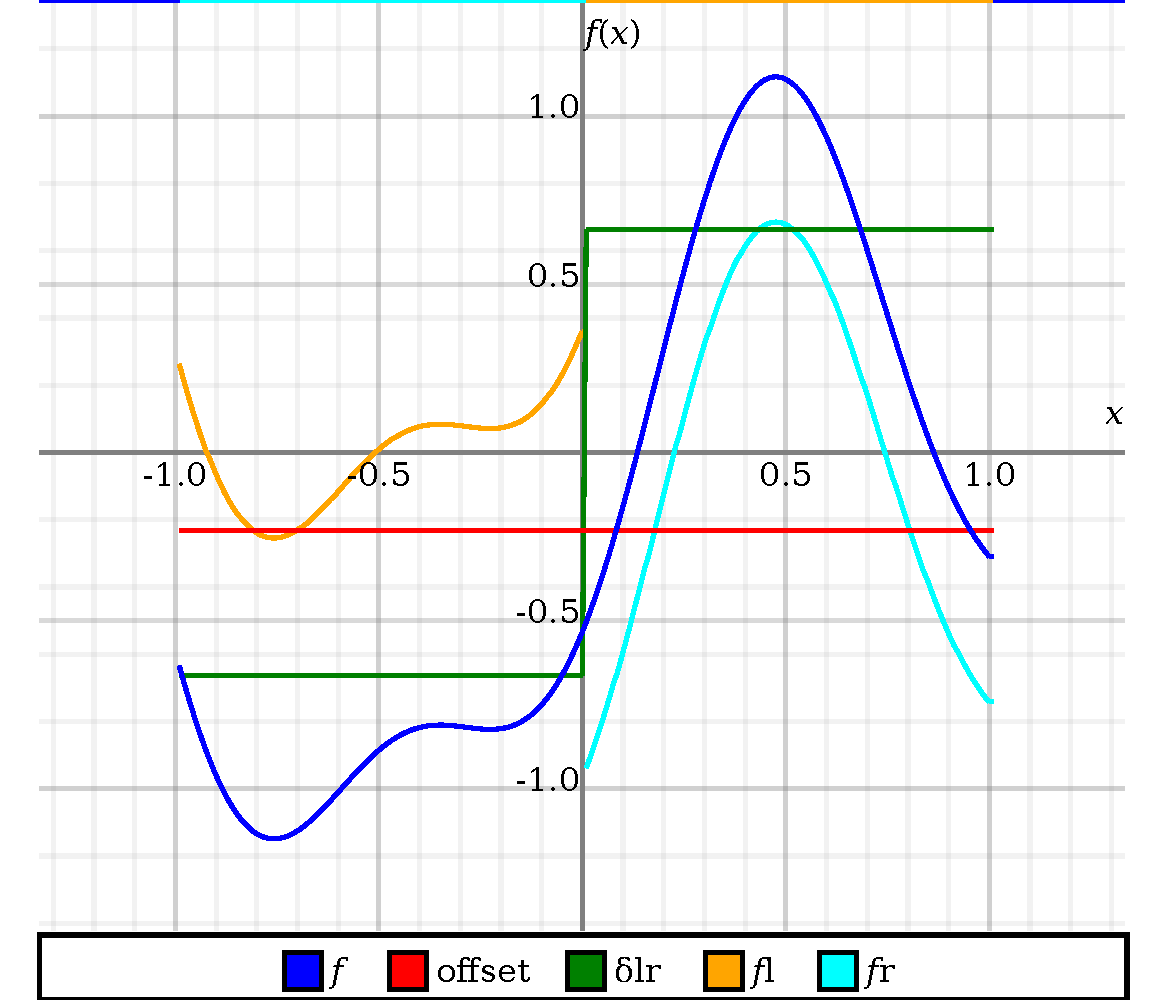
\includegraphics[width=\linewidth]{Haar-domDecompose.pdf}
 \caption{Example of how a function $f:D^1\to\mathbb{R}$ is decomposed into a constant offset, plus a step-function (Haar wavelet) for the offset-difference between left and right half, plus local fluctuations in each of the halves.}
 \label{haarDomDecompose}
\end{figure}
One can support functions with nonzero integral by simply adding an absolute offset with a wrapper-type at the top level:
\begin{lstlisting}
data Haar_D¹ y = Haar_D¹
    { global_offset :: !y
    , variation :: HaarUnbiased y }
\end{lstlisting}
The name “Haar” indicates that the basis functions of this data type (meaning those functions represented when exactly one of the fields of type ℝ in the \lstinline`HaarUnbiased ℝ` structure is 1, all other zero) are exactly the unnormalised Haar wavelets.

\section{Integration}
Whether using traditional orthonormal-basis methods, or the domain-decomposition approach introduced in \autoref{mulScaleResoIntro},
the numerical representations are obtained from integrating the function on an interval.
If the function is given as an analytic expression, it might be possible to calculate this integral exactly,
but this is typically impossible, and one resorts to numerical approximations.
All such approximations amount to some weighted average of the sample points:
\[
  \int_{D^1}\!\mathrm{d}x\:f(x) \approx \sum_i w_i\cdot f(x_i)
\]
with $x_i\in D^1$, $\sum_i w_i = 1$.
% For the choice of evaluation points and weights there are many different considerations to achieve good accuracy efficiently, this shall not be discussed here.
The choice of the evaluation points $x_i$ and weights $w_i$ are subject to considerations of efficiency and accuracy which we will not discuss here.

Crucially for our purposes, the calculation can be split up across the domain just like the recursive \lstinline`HaarUnbiased` data structure is:
\[
  \int_{D^1}\!\mathrm{d}x\:f(x)
    = \frac12\int_{D^1}\!\mathrm{d}x\:f(\tfrac{x-1}2)
    + \frac12\int_{D^1}\!\mathrm{d}x\:f(\tfrac{x+1}2)
\]
Observe that $\tfrac{x-1}2$ only evaluates on the left-, $\tfrac{x+1}2$ only on the right half of the domain.

This allows constructing the \lstinline`HaarUnbiased` tree in single pass with bottom-up propagation of the partial integrals, to obtain the offset estimates at each level without redundant computation.
The choice of of numerical approximation only occurs at the smallest level;
the simplest possibility is to only evaluate it at a single point in the middle and give that full weight (rectangular method).
Thus the Haar representation can be obtained in $\mathcal{O}(n\cdot\log n)$ from a function on the interval:
\begin{lstlisting}
homsampleHaar_D¹ :: ( VectorSpace y
                    , Fractional (Scalar y) )
            => PowerOfTwo -> (D¹ -> y) -> Haar_D¹ y
homsampleHaar_D¹ (TwoToThe 0) f
   = Haar_D¹ (f 0) HaarZero
homsampleHaar_D¹ (TwoToThe i) f
   = case homsampleHaar_D¹ (TwoToThe $ i-1)
            <$> [ f . \x -> (x-1)/2
                , f . \x -> (x+1)/2 ] of
       [Haar_D¹ y0l sfl, Haar_D¹ y0r sfr]
        -> Haar_D¹ ((y0l+y0r)/2)
             $ HaarUnbiased ((y0r-y0l)/2) sfl sfr
\end{lstlisting}
This algorithm is in DSP called a \emph{fast wavelet transform}, which starts out with a PCM-sampled array instead of a function-to-be-sampled.
One advantage of our approach is that it is not necessary to select one global maximum resolution (here the \lstinline`PowerOfTwo` parameter); instead, a heuristic can be added that refines the resolution \emph{locally} until the function is satisfactorily approximated.
\begin{remark}
Similar adaptive resolution strategies often dramatically improve performance in real-world applications, such as physics/engineering simulations (finite elements or finite volumes methods, where they correspond to adaptive mesh refinement).
It is also the main principle behind image compression formats which use quantization on a wavelet expansion.
The reason is that images or solutions to nonliner differential equations are often quite smooth in most of the domain, but include sharp edges / transients / shocks confined to a much smaller area.
\end{remark}

\section{Dual space: functionals}
The dual space of a function space $X$ consists of functions as well, but its domain is $X$ itself:
\begin{align*}
  X \subset& (D^1 \to \mathbb{R})
 \\
  X^\ast \subset& \bigl(X \to \mathbb{R}\bigr).
\end{align*}
In fact, $X$ consists of \emph{continuous, linear} functions, also called \emph{functionals}.
Although the space of functionals may initially seem much “bigger” than the space of functions,
in the case of $X$ being a Hilbert space, $X^\ast$ is in fact isomorphic to $X$ (Riesz representation theorem).
Of course, a crucial argument for this is that $X^\ast$ includes only continuous, linear functions.

% But actually, even simple-looking linear functionals do not typically correspond to functions in $X$. In particular, there are two conspicuous classes of linear functionals which cannot both be mapped to functions in a consistent way:
% \begin{itemize}
%  \item Evaluation at a single point (or a discrete collection of points). % Add example formula
%  \item Integration over an interval.  % +example
% \end{itemize}
% The reason that this does not contradict the Riesz theorem is that the standard Hilbert spaces of functions actually contain \emph{equivalence classes} of functions, rather than individual functions. In the $\mathcal{L}^2$ space, functions which differ only in a single point are considered the same vector.
Note that in the case of $X = \mathcal{L}^2$, evaluation at a single point is not an element of $X^{\ast}$, as it cannot be defined in a consistent manner.

On one hand, this can be physically motivated (limited precision, so it would never be possible to focus an experiment on a single point anyway).
On the other hand, theoretical physics is actually thrive with calculations that do involve single-point evaluations.
Mathematically, this just has to do with a judicious choice of function space.

Pointwise evaluation corresponds to a distribution widely called \emph{Dirac distribution}, sometimes introduced informally as
\begin{align*}
  \delta &:\quad \mathbb{R} \to “\mathbb{R}\cup\{\infty\}”
 \\
  \delta(x) &= \begin{cases} “\infty” & \text{if }x=0
                          \\ 0        & \text{otherwise} \end{cases}.
\end{align*}
As a distribution, however, its definition is perfectly clear:
\begin{align*}
  \delta^\ast &:\quad (\mathbb{R} \to \mathbb{R}) \to \mathbb{R}
 \\
  \delta^\ast(f) &= f(0).
\end{align*}
\begin{remark}
The previous equation is sometimes written informally as
\[
  \delta^\ast(f) = \int_\mathbb{R}\!\mathrm{d}x\: \delta(x)\cdot f(x),
\]
as if $\delta$ was a function.
\end{remark}

In the common fixed-finite resolution PCM discretisation, the Dirac distribution can be replaced by a function \emph{without} requiring an “infinite peak”.
As the smallest feature that can ever be resolved has a size at least $h$,
all features are \emph{only} characterised by the integral over an interval of that width,
corresponding to the following approximation of $\delta$:
\begin{align*}
  \delta_h &:\quad \mathbb{R} \to \mathbb{R}
 \\
  \delta_h(x) &= \begin{cases} \frac1h & \text{if }|x|<\tfrac{h}2
                          \\ 0         & \text{otherwise} \end{cases}
\end{align*}
% is in that case equivalent to the unrigorous-but-exact definition including an infinity.
The problem with this is that it is still necessary to know the resolution a priori.
Furthermore, too low estimates produce inaccurate results,
while too high ones unnecessarily increase the computational burden.

We therefore argue that PCM or other fixed-resolution approaches are not suitable for problems involving Dirac point-distributions (e.g., point masses in a gravity simulation).
It turns out that the \lstinline`Haar_D¹` tree structure has a representation of the dual space which includes Dirac distribution \emph{exactly},
as well as distributions spread across an interval.

The idea is to mirror the tree data structure (as Riesz suggests),
but instead of using a Hilbert space inner product,
we simply read off the stored coefficients as they are.
One could argue that these coefficients are “unphysical” because via the Haar wavelets they represent differences rather than actual sample values\footnote{%
This would anyways be hypocritical, since in a fixed-resolution discretisation of $\mathcal{L}^2$ the coefficients \emph{also} don't strictly speaking correspond to concrete sample values, but rather to an integral over such values or even, in the Shannon-Nyquist derivation, to a discrete IFT of the truncation of the infinite sequence of Fourier coefficients.
} but in fact, both the function-space type and its dual are intended to be used as abstract vector spaces with no public way to directly access the coefficients of either.

Notice that the trees now need \emph{not} have finite depth,
because there is no reason to evaluate a distribution at a single point as with \lstinline`evalPreIntg_D¹`,
but only as a functional with a whole function,
which is already required to have only a finite feature-resolution.
Thus the tree can now be non-strict,
\begin{lstlisting}
data CoHaarUnbiased y
     = CoHaarZero
     | CoHaarUnbiased !y (HaarUnbiased y)
                         (HaarUnbiased y)
data CoHaar_D¹ y
     = CoHaar_D¹ !y (CoHaarUnbiased y)
\end{lstlisting}
but because \lstinline`HaarUnbiased` is strict the functional evaluation is still guaranteed to terminate\footnote{%
This is in striking analogy with the Agda programming language, in which data types are strict by default but there is also \emph{co-data} (coinductive types) allowing for infinite streams.
}:
\begin{lstlisting}
(<.>^) :: CoHaar_D¹ ℝ -> Haar_D¹ ℝ -> ℝ
CoHaar_D¹ q0 qFluct <.>^ Haar_D¹ f0 fFluct
    = q0 * f0 + qFluct~<.>^fFluct
 where CoHaarZero ~<.>^ _ = 0
       _ ~<.>^ HaarZero = 0
       CoHaarUnbiased δq ql qr
            ~<.>^ HaarUnbiased δf fl fr
          = δq * δf + ql~<.>^fl + qr~<.>^fr
\end{lstlisting}
note that \emph{no} scaling/normalisation is performed
(as would be the case if this were an integral-based inner product)
as the recursive call zooms into the left and right subinterval.

We are now in a position to construct a functional for which \lstinline`<.>^` evaluates the integral over an arbitrary interval:
we regard the function as decomposed on the subdomains,
but instead of accepting a \lstinline`Haar_D¹` value,
% we record in the dual vector with what weight its coefficients would be used in the result:
we record the weights of the dual vector:
\todo[inline, author=OV]{This makes no sense}
\begin{lstlisting}
boxDistribution :: (D¹, D¹)  -- ^ Target interval
                -> ℝ         -- ^ Total weight
                -> Haar_D¹ DistributionSpace ℝ
boxDistribution (D¹ l, D¹ r) y
  | l > r      = boxDistribution (D¹ r, D¹ l) y
boxDistribution (D¹ (-1), D¹ 1) y
               = CoHaar_D¹ y zeroV
boxDistribution (D¹ l, D¹ r) y
  | l<0, r>0  -- intersecting both halves of domain
      = CoHaar_D¹ y $ CoHaarUnbiased (wr-wl) lstru rstru
  | l<0       -- target intersects only left half
      = CoHaar_D¹ y $ CoHaarUnbiased  (-wl)  lstru 0
  | otherwise -- target intersects only right half
      = CoHaar_D¹ y $ CoHaarUnbiased   wr    0   rstru
 where CoHaar_D¹ wl lstru = boxDistribution
                      (D¹ $ l*2 + 1, D¹ $ min 0 r*2 + 1)
                      (y * if r>0 then l/(l-r) else 1)
       CoHaar_D¹ wr rstru = boxDistribution
                      (D¹ $ max 0 l*2 - 1, D¹ $ r*2 - 1)
                      (y * if l<0 then r/(r-l) else 1)
\end{lstlisting}
The tree generated this way will in general have infinite depth in order to select the desired interval with any delimiters.
However, the distribution will only narrow in on this selection provided that the function on which we evaluate has any structure at that level.
When the function is eventually constant, only the top-level coefficient is evaluated (as that corresponds to the integral, which is what is sought here).

Furthermore, \lstinline`boxDistribution` itself only builds up the infinitely fine resolution where it is actually required, i.e., at the \emph{boundaries} of the target interval:
on those subdivisions that are fully in the interval, again only to top-level coefficient of the function needs to be evaluated, whereas outside of the target the result will simply be zero.
Thus, the tree has only two long branches, and \lstinline`<.>^` has only a complexity of $\mathcal{O}(\log n)$ in the resolution of the function which the distribution is contracted against.
(Compare this with a PCM implementation, where a box distribution would need to contain $\mathcal{O}(n)$ nonzero entries, all of which would need to be evaluated.)

Remarkably, all of this works even if the target “interval” actually has zero width:
\begin{lstlisting}
dirac :: D¹ -> CoHaar_D¹ ℝ
dirac x0 = boxDistribution (x0,x0) 1
\end{lstlisting}

That implementation of the Dirac distribution does indeed evaluate functions of arbitrary resolution at one point.
As tested with QuickCheck,
\begin{lstlisting}
  testProperty "Dirac eval of Haar function"
   $ \f p -> dirac p<.>^f ~= evalHaarFunction f p
\end{lstlisting}
where the QuickCheck \lstinline`Arbitrary` instance generates arbitrarily deep tree structures, and picks any point on $D^1$ for evaluation.
\lstinline`~=` checks equality up to floating-point inaccuracy (in our test suite, the relative error  is set to $10^{-9}$).

\section{Tensor products and linear maps}
Perhaps most important aspect about the dual space is that it gives rise to a storable implementation of arbitrary linear mappings.
\begin{lstlisting}
newtype LinearMap v w = LinearMap
           (TensorProduct (DualVector v) w)
\end{lstlisting}
The \lstinline`TensorProduct` for a parameterised type like \lstinline`Haar_D¹` and \lstinline`CoHaar_D¹` -- generally, for any functor in the category of vector spaces%
\footnote{They are in fact also functors in the \textbf{Hask} category, but we recommend keeping that instance a private implementation detail because fmapping a nonlinear function is not invariant of the choice of basis, i.e. it is not safe with respect to refactoring to another representations.
} -- is simply given by instantiating the parameter with the right factor space.
\begin{lstlisting}
type instance Scalar y ~ ℝ
   => TensorProduct (CoHaar_D¹ ℝ) w = CoHaar_D¹ w
\end{lstlisting}
So specifically, \lstinline`LinearMap (Haar_D¹ ℝ) (Haar_D¹ ℝ)` is represented by a distribution of functions, i.e. by of the type \lstinline`CoHaar_D¹ (Haar_D¹ ℝ)`.
This type is important because it would be the type of the identity linear mapping, which is required for \lstinline`Haar_D¹ ℝ` to be a member of of an actual category and prerequisite for generalising several linear algebra algorithm from the finite-Euclidean case to infinite-dimensional spaces like \lstinline`Haar_D¹ ℝ`.
This is another reason why \lstinline`CoHaar_D¹` must be non-strict: the identity mapping must use an infinite tree, namely
\begin{lstlisting}
id :: LinearMap (Haar_D¹ ℝ) (Haar_D¹ ℝ)
id = LinearMap $ CoHaar_D¹
           (Haar_D¹ 1 zeroV)
           (fmap (\ δ -> Haar_D¹ 0 δ) idUnbiased)
 where idUnbiased :: TensorProduct (CoHaarUnbiased ℝ)
                                   (HaarUnbiased ℝ)
       idUnbiased = CoHaarUnbiased
        (CoHaar_D¹ 1 zeroV zeroV)
        (fmap (\l -> HaarUnbiased 0 l zeroV) idUnbiased)
        (fmap (\r -> HaarUnbiased 0 zeroV r) idUnbiased)
\end{lstlisting}

%% Acknowledgments
\begin{acks}                            %% acks environment is optional
                                        %% contents suppressed with 'anonymous'
  %% Commands \grantsponsor{<sponsorID>}{<name>}{<url>} and
  %% \grantnum[<url>]{<sponsorID>}{<number>} should be used to
  %% acknowledge financial support and will be used by metadata
  %% extraction tools.
  This material is based upon work supported by the
  \grantsponsor{GS100000001}{National Science
    Foundation}{http://dx.doi.org/10.13039/100000001} under Grant
  No.~\grantnum{GS100000001}{nnnnnnn} and Grant
  No.~\grantnum{GS100000001}{mmmmmmm}.  Any opinions, findings, and
  conclusions or recommendations expressed in this material are those
  of the author and do not necessarily reflect the views of the
  National Science Foundation.
\end{acks}


%% Bibliography
%\bibliography{bibfile}


%% Appendix
\appendix
\section{Appendix}

Text of appendix \ldots

\end{document}
